\clearpage

\section{Decoder}

This block accepts a complex electrical signal and outputs a sequence of binary values (0's and 1's). Each point of the input signal corresponds to a pair of bits.

\subsection*{Input Parameters}

\begin{itemize}
	\item\texttt{t\_integer} m\{ 4 \}
	\item vector$<$\texttt{t\_complex}$>$ iqAmplitudes\{ \{ 1.0, 1.0 \},\{ -1.0, 1.0 \},\{ -1.0, -1.0 \},\{ 1.0, -1.0 \} \};
\end{itemize}

\subsection*{Methods}
 
Decoder() {}
\bigbreak
Decoder(vector$<$Signal *$>$ \&InputSig, vector$<$Signal *$>$ \&OutputSig) :Block(InputSig, OutputSig) {}
\bigbreak
void initialize(void)
\bigbreak
bool runBlock(void)
\bigbreak
void setM(int mValue)
\bigbreak
void getM()
\bigbreak
void setIqAmplitudes(vector$<$\texttt{t\_iqValues}$>$ iqAmplitudesValues)
\bigbreak
vector$<$\texttt{t\_iqValues}$>$getIqAmplitudes()

\subsection*{Functional description}

This block makes the correspondence between a complex electrical signal and pair of binary values using a predetermined constellation.

To do so it computes the distance in the complex plane between each value of the input signal and each value of the \textit{iqAmplitudes} vector selecting only the shortest one. It then converts the point in the IQ plane to a pair of bits making the correspondence between the input signal and a pair of bits.

\pagebreak

\subsection*{Input Signals}

\subparagraph*{Number:} 1

\subparagraph*{Type:} Electrical complex (TimeContinuousAmplitudeContinuousReal)

\subsection*{Output Signals}

\subparagraph*{Number:} 1

\subparagraph*{Type:} Binary 

\subsection*{Examples}

As an example take an input signal with positive real and imaginary parts. It would correspond to the first point of the \textit{iqAmplitudes} vector and therefore it would be associated to the  pair of bits $00$. 

\begin{figure}[h]
	\centering
	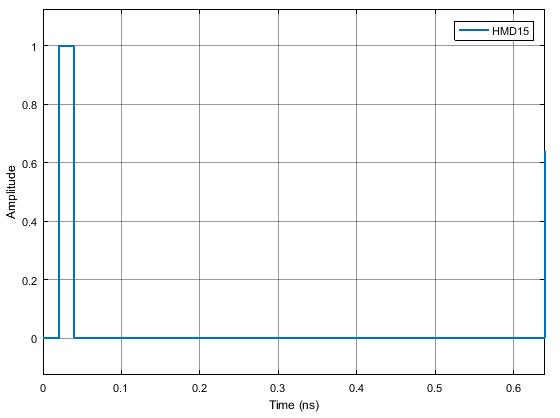
\includegraphics[width=\textwidth]{../homodyne_receiver/figures/Decoder_output}
	\caption{Example of the output signal of the decoder for a binary sequence 01. As expected it reproduces the initial bit stream}\label{Decoder_output}
\end{figure}

\subsection*{Sugestions for future improvement}
